\documentclass[11pt]{article}

%\usepackage{palatino}

\usepackage[utf8]{inputenc}
\usepackage[T1]{fontenc}
% Chivo como en las diapositivas o Fira Sans?
%\usepackage[familydefault,regular]{Chivo}
\usepackage[sfdefault,scaled=.85]{FiraSans}
\usepackage{newtxsf}
\usepackage{mathastext}
\usepackage[spanish]{babel}
\setlength{\parindent}{0pt}
\usepackage{amssymb}
\usepackage{amsmath}
\usepackage{wasysym}
\usepackage[x11names, rgb, html]{xcolor}
\usepackage{graphics}
\usepackage{caption}
\usepackage{lipsum}
\usepackage{float}
\usepackage{adjustbox}
\usepackage{geometry}
\usepackage[scaled=.85]{FiraMono}
\usepackage{algpseudocode}
\usepackage{algorithm}

\geometry{left=3cm,right=3cm,top=3cm,bottom=3cm,headheight=1cm,headsep=0.5cm}

%%% PGFPLOTSTABLE

\usepackage{pgfplotstable}

%%% COLORES

\definecolor{50}{HTML}{FFEBEE}
\definecolor{100}{HTML}{FFCDD2}
\definecolor{200}{HTML}{EF9A9A}
\definecolor{300}{HTML}{E57373}
\definecolor{400}{HTML}{EF5350}
\definecolor{500}{HTML}{F44336}
\definecolor{600}{HTML}{E53935}
\definecolor{700}{HTML}{D32F2F}
\definecolor{800}{HTML}{C62828}
\definecolor{900}{HTML}{B71C1C}



%% Colores de Solarized

\definecolor{sbase03}{HTML}{002B36}
\definecolor{sbase02}{HTML}{073642}
\definecolor{sbase01}{HTML}{586E75}
\definecolor{sbase00}{HTML}{657B83}
\definecolor{sbase0}{HTML}{839496}
\definecolor{sbase1}{HTML}{93A1A1}
\definecolor{sbase2}{HTML}{EEE8D5}
\definecolor{sbase3}{HTML}{FDF6E3}
\definecolor{syellow}{HTML}{B58900}
\definecolor{sorange}{HTML}{CB4B16}
\definecolor{sred}{HTML}{DC322F}
\definecolor{smagenta}{HTML}{D33682}
\definecolor{sviolet}{HTML}{6C71C4}
\definecolor{sblue}{HTML}{268BD2}
\definecolor{scyan}{HTML}{2AA198}
\definecolor{sgreen}{HTML}{859900}

%% Colores del documento

\definecolor{text}{RGB}{78,78,78}
\definecolor{accent}{RGB}{129, 26, 24}

%%% LISTINGS

\usepackage{listingsutf8}

%% Las tildes

\lstset{
  inputencoding=utf8/latin1
}

%% Colores de Solarized para listings

\lstset{
  % How/what to match
  % sensitive=true,
  % language=pseudo,
  % Border (above and below)
  frame=leftline,
  rulecolor=\color{300},
  framerule=2pt,
  % Line number
  numbers=left,
  % Extra margin on line (align with paragraph)
  xleftmargin=\parindent,
  % Put extra space under caption
  belowcaptionskip=1\baselineskip,
  % Colors
  % backgroundcolor=\color{sbase3},
  basicstyle=\footnotesize\ttfamily\color{sbase00},
  keywordstyle=\color{700},
  commentstyle=\color{300},
  stringstyle=\color{500},
  numberstyle=\color{500},
  %identifierstyle=\color{500},
  % Break long lines into multiple lines?
  breaklines=true,
  % Show a character for spaces?
  showstringspaces=false,
  tabsize=2,
  xleftmargin=0.7em,
}

\renewcommand{\lstlistingname}{Código fuente}% Listing -> Algorithm


\title{Algorítmica: práctica 3 \\ \large Recubrimiento de un grafo no dirigido\\ \vspace{0.2em}Grupo 2}
\author{Sofía Almeida Bruno \and Antonio Coín Castro \and María Victoria Granados Pozo \and Miguel Lentisco Ballesteros \and José María Martín Luque}
\date{\today}

\begin{document}
\maketitle

\newpage

\section*{Análisis del problema}

Dado un grafo no dirigido $G=(V,E)$, un conjunto $U\subseteq V$ es un recubrimiento de $G$ si cada arista de $E$ incide en, al menos, un vértice o nodo de $U$. Nuestro problema consiste en encontrar un recubrimiento minimal del grafo $G$, esto es, un recubrimiento con el menor número posible de nodos. \\

Para resolver el problema, empleamos un algoritmo \textit{greedy} (voraz). La solución que proporcionamos es el conjunto de nodos que forman el recubrimiento junto con el coste (número de nodos). \\

Para representar nuestro problema, hemos usado una clase \verb|Problema| y una clase \verb|Solucion|. En \verb|Problema| se encapsula la matriz de adyacencia del grafo (simétrica) junto con su tamaño, mientras que en \verb|Solucion| se encapsula un vector de nodos que forman el recubrimiento, junto a su tamaño. Se adjunta el código fuente de ambas clases.\\

\begin{figure}[H]
	\caption{Ejemplo de grafo. Los nodos más oscuros forman un recubrimiento}
	\centering 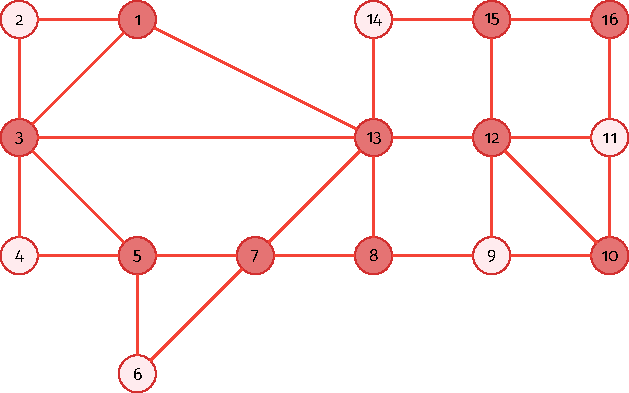
\includegraphics{./img/grafo.pdf}
\end{figure}

\section*{Diseño de la solución}

Empleando un enfoque \textit{greedy} para la resolución del problema, la idea es ir seleccionando para el recubrimiento los nodos del grafo que tienen el mayor número de incidencias. El número de incidencias de un nodo (número de aristas que tienen a ese nodo como extremo) se conoce también como \textit{grado del nodo}. \\

En primer lugar, vamos a mostrar las componentes Greedy de este problema:

\begin{itemize}
	\item \textit{Lista de candidatos:} los nodos del grafo.
	\item \textit{Lista de candidatos utilizados:} los nodos ya considerados para el recubrimiento.
	\item \textit{Función solución:} que no haya ninguna arista sin considerar.
	\item \textit{Criterio de factibilidad:} que el nodo esté en la lista de candidatos (no es necesario ningún criterio adicional).
	\item \textit{Función objetivo:} recubrimiento de coste mínimo.
	\item \textit{Función de selección:} nodo en el que inciden más aristas.
\end{itemize}

Una vez que hemos visto las componentes, pasemos a ver un esqueleto o \textit{pseudocódigo} del algoritmo: \\

$N \equiv \text{ número de nodos del grafo}\\ M \equiv \text{ número de nodos del recubrimiento}\\ L \equiv \text{ matriz de adyacencia}\\ T[1,\dots,M] \equiv \text{ vector de nodos del recubrimiento}\\ V[1,\dots,N] \equiv \text{ vector de incidencias}$\\

\begin{algorithm}
\begin{algorithmic}


\Function{RecubrimientoGrafoGreedy }{$L[1,\dots,N][1,\dots,N]\ $}
    \State $T = \emptyset$ \Comment Recubrimiento
    \For{$i=1,\dots,N$}
        \State $\displaystyle V[i] \gets \sum_{j=1}^N L[i][j]$ \Comment Número de incidencias del nodo $i$
    \EndFor

    \State $p \gets \text{Nodo con más incidencias} \left( V[p] \ge V[i] \ \ \forall i \right)$ \Comment Función de selección \\

    \While{$V[p] > 0$} \Comment Función solución

        \State $T \gets T \cup \{p\}$
        \State $V[p] \gets 0$
        \For{$j=1,\dots,N$}
            \If{Están conectados $p$ y $j$ \textbf{and} $V[j] > 0$ }
                \State $V[j] \gets V[j]-1$
            \EndIf
        \EndFor
        \State $p \gets \text{Nodo con más incidencias} \left( V[p] \ge V[i] \ \ \forall i \right)$ \Comment Función de selección

    \EndWhile \\
    \State \Return $T$
\EndFunction
\end{algorithmic}
\end{algorithm}

Como se puede observar, algunas de las componentes \textit{greedy} listadas anteriormente se han omitido o modificado en la implementación, pues o bien no son necesarias, o bien es más sencillo implementarlas de otra manera.

\begin{itemize}
	\item La \textit{lista de candidatos} y la \textit{lista de candidatos utilizados} están representadas como un vector de incidencias $V$, donde si el nodo $i$ está utilizado, entonces $V[i] = 0$.
	\item El \textit{criterio de factibilidad}, como ya dijimos, no es necesario, pues todos los nodos de la \textit{lista de candidatos} son factibles. Implícitamente, estamos considerando como factibles los nodos $i$ tales que $V[i] > 0$.
	\item La \textit{función solución} es que el vector de incidencias $V$ sea distinto del vector $0$, o lo que es lo mismo, que el máximo de las componentes de $V$ no sea $0$. Esto significaría que ya se han considerado todas las aristas que inciden en cada uno de los nodos.
	\item La \textit{función de selección} consiste en seleccionar, en cada paso, la componente máxima del vector $V$, es decir, el nodo con mayor grado.
\end{itemize}

En el diseño del algoritmo nos aprovechamos del vector $V$ para identificar \textbf{cada nodo del grafo con cada posición de $V$}. Es decir, $V[i]$ representa el número de incidencias del nodo $i$.

\section*{Algoritmo Greedy}

Veamos ahora el algoritmo implementado en el lenguaje \verb|C++|. En primer lugar, hemos separado la implementación de la \textit{función de selección}, para que se aprecie con claridad:

	\lstinputlisting[language=C++, linerange={12-24}, caption=Función de selección]{./../src/Algoritmo.cpp}
\vspace{1em}

Ahora pasemos a la función principal. El algoritmo comienza construyendo un vector de incidencias, que contiene en cada posición $i$ el número de aristas que inciden en el nodo $i-$ésimo. Después, seleccionamos el nodo con un número mayor de incidencias, lo añadimos a la solución y eliminamos las aristas que inciden en dicho nodo. A efectos prácticos, esto consiste en poner a $0$ el número de incidencias del nodo en $V$, y en decrementar en $1$ el número de incidencias de los nodos conectados con él.\\


El algoritmo continúa repitiendo el paso anterior hasta que no quedan aristas sin considerar (notemos que no volverá a seleccionar nunca un nodo ya considerado). Cuando finalice el algoritmo, tendremos como solución un vector con los nodos utilizados en el recubrimiento, y el coste será el número de nodos del mismo.\\

\lstinputlisting[language=C++, linerange={25-59}, caption=Algoritmo Greedy]{./../src/Algoritmo.cpp}

La solución \verb|sol| utilizada es una instacia de la clase \verb|Solucion|, que contiene un vector con los nodos y su tamaño. Esta función \verb|RecubrimientoGrafoGreedy| recibe como parámetro un objeto $p$ de la clase \verb|Problema| que encapsula la matriz de adyacencia del grafo en cuestión, donde se ven reflejadas indirectamente las incidencias de cada nodo.

\section*{Ejemplo paso a paso}
%% FIXME ARREGLAR FORMATO
Vamos a ver con un grafo concreto cómo funciona el algoritmo. Consideremos el siguiente grafo.

\begin{figure}[H]
	\caption{Ejemplo de grafo sin recubrir}
	\centering 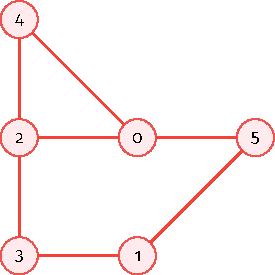
\includegraphics{./img/grafo-ejemplo-sin-recubrir.pdf}
\end{figure}

Inicialización:\\
%% FIXME centrar o poner esto de una forma adecuada
N = \verb|num_nodos| = 6

M = \verb|sol.coste| = 0

$$  L = \verb|p.matriz_adyacencia| =
\begin{pmatrix}
	0 & 0 & 1 & 0 & 1 & 1 \\
	0 & 0 & 0 & 1 & 0 & 1 \\
	1 & 0 & 0 & 1 & 1 & 0 \\
	0 & 1 & 1 & 0 & 0 & 0 \\
	1 & 0 & 1 & 0 & 0 & 0 \\
	1 & 1 & 0 & 0 & 0 & 0
\end{pmatrix}$$

$$ V = \verb|incidencias| =
\begin{pmatrix}
	3 \\
	2 \\
	3 \\
	2 \\
	2 \\
	2
\end{pmatrix}$$

p = \verb|pos_max| = 0\\

Bucle \verb|while|:

\verb|incidencias[0]| = 3 > 0, entra en el bucle\\
Añadimos el nodo 0 al vector solución. T = \verb|sol.nodos| = \{0\}.
M = \verb|sol.coste| = 1\\

\begin{figure}[H]
	\centering 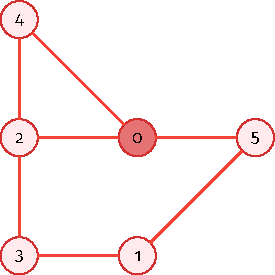
\includegraphics{./img/grafo-ejemplo-1.pdf}
\end{figure}

Actualizamos el vector de incidencias, eliminando a este nodo y las incidencias correspondientes. Como las aristas adyacentes al nodo 0 inciden también en los nodos 2, 4 y 5, restamos uno en dichas posiciones del vector de incidencias: \\
$$ V = \verb|incidencias| =
\begin{pmatrix}
	3 \\
	2 \\
	3 \\
	2 \\
	2 \\
	2
\end{pmatrix} \implies V = \verb|incidencias| =
\begin{pmatrix}
	0 \\
	2 \\
	2 \\
	2 \\
	1 \\
	1
\end{pmatrix}$$
Restablecemos el valor de p = \verb|pos_max| = 1

Como \verb|incidencias[1]| = 2 > 0, realiza otra iteración de forma similar:\\

 T = \verb|sol.nodos| = \{0, 1\}, M = \verb|sol.coste| = 2, las aristas que inciden en el nodo 1 lo hacen también en los nodos 3 y 5.\\

\begin{figure}[H]
	\centering 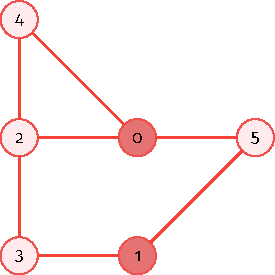
\includegraphics{./img/grafo-ejemplo-2.pdf}
\end{figure}

$$ V = \verb|incidencias| =
\begin{pmatrix}
	0 \\
	2 \\
	2 \\
	2 \\
	1 \\
	1
\end{pmatrix} \implies V = \verb|incidencias| =
\begin{pmatrix}
	0 \\
	0 \\
	2 \\
	1 \\
	1 \\
	0
\end{pmatrix}$$

Volvemos a actualizar el valor de p = \verb|pos_max| = 2.\\
\verb|incidencias[1]| = 2 > 0, por tanto, repetimos el proceso una vez más: T  = \verb|sol.nodos| = \{0, 1, 2\}.
M = \verb|sol.coste| = 3.

\begin{figure}[H]
	\centering 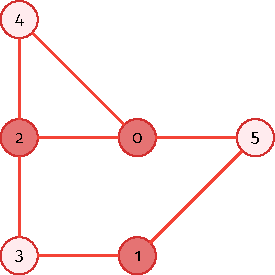
\includegraphics{./img/grafo-ejemplo.pdf}
\end{figure}

Eliminando las incidencias de las aristas adyacentes a este nodo el vector de incidencias sufre el siguiente cambio:

 $$ V = \verb|incidencias| =
\begin{pmatrix}
	0 \\
	0 \\
	2 \\
	1 \\
	1 \\
	0
\end{pmatrix} \implies V = \verb|incidencias| =
\begin{pmatrix}
	0 \\
	0 \\
	0 \\
	0 \\
	0 \\
	0
\end{pmatrix}$$

 p = \verb|pos_max| = 0, por tanto, \verb|incidencias[1]| = 0 == 0, no entra en bucle while. Como último paso devolvemos la solución:  T  = \verb|sol.nodos| = \{0, 1, 2\}, M = \verb|sol.coste| = 3.

\section*{Eficiencia teórica}
La eficiencia del algoritmo viene dada por el bucle \textit{while}. Este bucle se ejecutará hasta que todos los valores del vector de incidencias sean $0$, que en el peor de los casos es el número total de nodos menos 1 $(N - 1)$.\\

En el interior de este bucle, lo que determina la eficiencia es la \textit{función de selección}, que como tiene que recorrer el vector $V$ es de orden $N$. Por tanto la eficiencia de este algoritmo es $N(N-1) = N^2 - N$. Notemos que el bucle \textit{for} dentro del \textit{while} tiene el mismo orden de eficiencia que la función de selección.\\

Es decir, si llamamos $V$ al conjunto de nodos del grafo, la eficiencia del algoritmo es $O(|V|^2)$.

\section*{Optimalidad}

Hemos notado que nuestro algoritmo no es óptimo, es decir, no siempre nos proporciona un recubrimiento minimal. Sin embargo, siempre es posible encontrar una solución, aunque sea la trivial (a saber, un recubrimiento formado por $N-1$ nodos).\\

Veamos con un contraejemplo que nuestro algoritmo puede proporcionarnos un recubrimiento que no es óptimo. Consideremos el siguiente grafo:

\begin{figure}[H]
	\centering 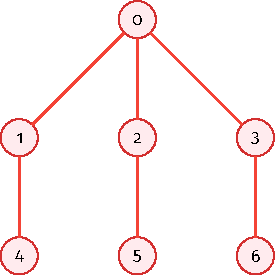
\includegraphics{./img/grafo2.pdf}
\end{figure}

Es obvio que el recubrimiento minimal de este grafo sería el siguiente:

\begin{figure}[H]
	\centering 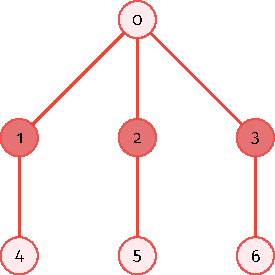
\includegraphics{./img/grafo2-minimal.pdf}
\end{figure}

Sin embargo, como nuestro algoritmo selecciona en primer lugar los nodos de mayor grado, seleccionaría al comienzo el nodo $0$, lo que ya condiciona a que el recubrimiento obtenido sea el siguiente, que no es minimal:

\begin{figure}[H]
	\centering 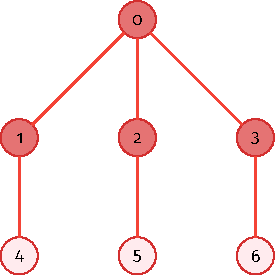
\includegraphics{./img/grafo2-no-minimal.pdf}
\end{figure}

\section*{Problema real de recubrimiento}

Supongamos un grafo no dirigido en el que los nodos representan diversas ciudades, y las aristas las carreteras que las unen. Además, entre una ciudad y otra hay varios pueblos.\\

El dueño de una conocida empresa de fabricación de marcapáginas quiere extender su red de tiendas en esta región, de tal forma que se cumplan los siguientes requisitos:

\begin{itemize}
    \item Solo se pueden abrir tiendas de marcapáginas en las ciudades.
	\item Los habitantes de las ciudades deben poder adquirir un marcapáginas (porque leen mucho) sin tener que desplazarse más de una ciudad por carretera.
	 \item Los habitantes de los pueblos deben poder comprar un marcapáginas (también leen mucho) en una de las dos ciudades entre las que se encuentran.
\end{itemize}

Bajo estas condiciones, el problema se reduce a encontrar un recubrimiento minimal del grafo en cuestión.

\section*{Compilación y ejecución del proyecto}
Para compilar este proyecto simplemente hay que situarse en la carpeta \verb|p3_greedy| y ejecutar el comando make.\\

Una vez compilado, si estamos situados en la misma carpeta ejecutamos \verb|./bin/main| pasando como parámetro cualquiera de los archivos \verb|.dat| de la carpeta \verb|datos|.


\end{document}
